\documentclass[10pt, conference, compsocconf]{IEEEtran}

\usepackage{capt-of}
\usepackage{graphicx}
\usepackage{subfig}
\usepackage{booktabs}
\usepackage{multirow}
\usepackage{siunitx}
\usepackage{multicol}
\usepackage{array}
\usepackage{amsmath}
\newcommand{\nltable}[2][c]{%
  \begin{tabular}[#1]{@{}c@{}}#2\end{tabular}}
\newcommand{\wave}{\raise.17ex\hbox{$\scriptstyle\mathtt{\sim}$}}

\newcolumntype{C}[1]{>{\centering\let\newline\\\arraybackslash}m{#1}}

\begin{document}
\bstctlcite{IEEEexample:BSTcontrol}

\title{Approach of Matrix Multiplication on Cloud Distributed System}


\author{\IEEEauthorblockN{Myungjun Son}
\IEEEauthorblockA{Department of Computer Science\\
Kookmin University\\
Seoul, South Korea\\
smj8612@kookmin.ac.kr}
\and
\IEEEauthorblockN{Kyungyong Lee}
\IEEEauthorblockA{Department of Computer Science\\
Kookmin University\\
Seoul, South Korea\\
leeky@kookmin.ac.kr}
}

% make the title area
\maketitle

\begin{abstract}
  Matrix multiplication is an important kernel in many machine learning algorithms. As the size of input dataset increases, many workloads are analyzed on a large-scale distributed cloud computing environment, and understanding the characters of distributed matrix multiplication tasks is crucial for building an efficient environment. In this work, we propose MPEC, Matrix Multiplication Performance Estimator on Cloud Computing, that predicts the latency of various sizes and shapes of matrix multiplication on a distributed computing environment. We first characterize the workload overheads and propose eight features to model the latency with distinct input matrix types. Using the features, the prediction and parameter optimization are performed iteratively. By experimenting over 237 cases of distinct types of matrix multiplications on diverse cloud instance types on Spark, we confirm that the proposed method is effective in modeling the latency of various cases while modeling non-linear interactions among the proposed features. MPEC model's relative error shows 17\% and comparison with the state-of-the-art cloud computing performance predictor presents that MPC provides 16\% more accuracy and confirms the uniqueness of the distributed matrix multiplication workload. 
\end{abstract}

\IEEEpeerreviewmaketitle

\section{Introduction}\label{sec:intro}
Big data analytics systems are deployed in cloud computing environments to process ever-increasing dataset while guaranteeing stable operations; scalability and fault-tolerance from the perspective of infrastructure. To satisfy application demands from distinct use cases, cloud computing service providers offer various types of instances that applications can run. Using those resources, most big data platforms are deployed in a scale-out manner. As managing distributed datasets and tasks running on large-scale machines are challenging, abstractions of distributed datasets and resources are crucial to let application developers focus on tasks that really matter. Many systems are proposed to provide a simple and easy interface to handle large-scale datasets, to name a few, Hadoop~\cite{hadoop}, Spark~\cite{spark}, and recently TensorFlow~\cite{tensorflow}.

To extract valuable insights from a massive dataset, matrix multiplication is widely used. In recommendation systems, for example, the core computation kernel of matrix factorization algorithms, such as SVD and NMF~\cite{nmf}, is matrix-matrix multiplication. The matrix-vector multiplication is the core kernel in page-rank algorithm when using the power method to get principle eigen vectors~\cite{pagerank}. In order to build a cost efficient cloud environment that runs data mining tasks with distributed matrix computation kernel, it is crucial to estimate the kernel task overhead on different cloud computing instances with distinct matrix size. 

To understand the characteristics of matrix multiplication performance on a distributed cloud computing environment, we analyzed the performance of dense matrix multiplication with diverse input sizes and formations on distinct cloud computing instances. In the experiments, we multiply two square matrices with the number of rows being 10000, 20000, and 30000 on AWS EC2 \textit{R4, T2, M4, C4, G2} instances with a size of \textit{2xlarge}. We use Apache Spark MLLib BlockMatrix library~\cite{spark-mm} to conduct the experiments with four machines that have OpenBlas installed. 

Figure~\ref{fig:different-instance-types} shows the normalized latency to the fastest completing instance type in the gray bar. As shown in the figure, as the input matrix size differs, the best performing instance type also differs - no globally optimal instance type. If we consider the price factor of each instance, the performance difference even gets bigger as shown in the red star mark. Furthermore, as shown in the Figure~\ref{fig:instance-blocks-sizes-compare}, multiplying two non-square matrices shows significantly different performance comparing to the square matrix multiplication though the number of compute operation is the same - i.e., the number of (left matrix rows $\times$ left matrix columns $\times$ right matrix columns).

\begin{figure}[t]
  \centering
  \subfloat[Performance of different instance types of 2xlarge]{\label{fig:different-instance-types}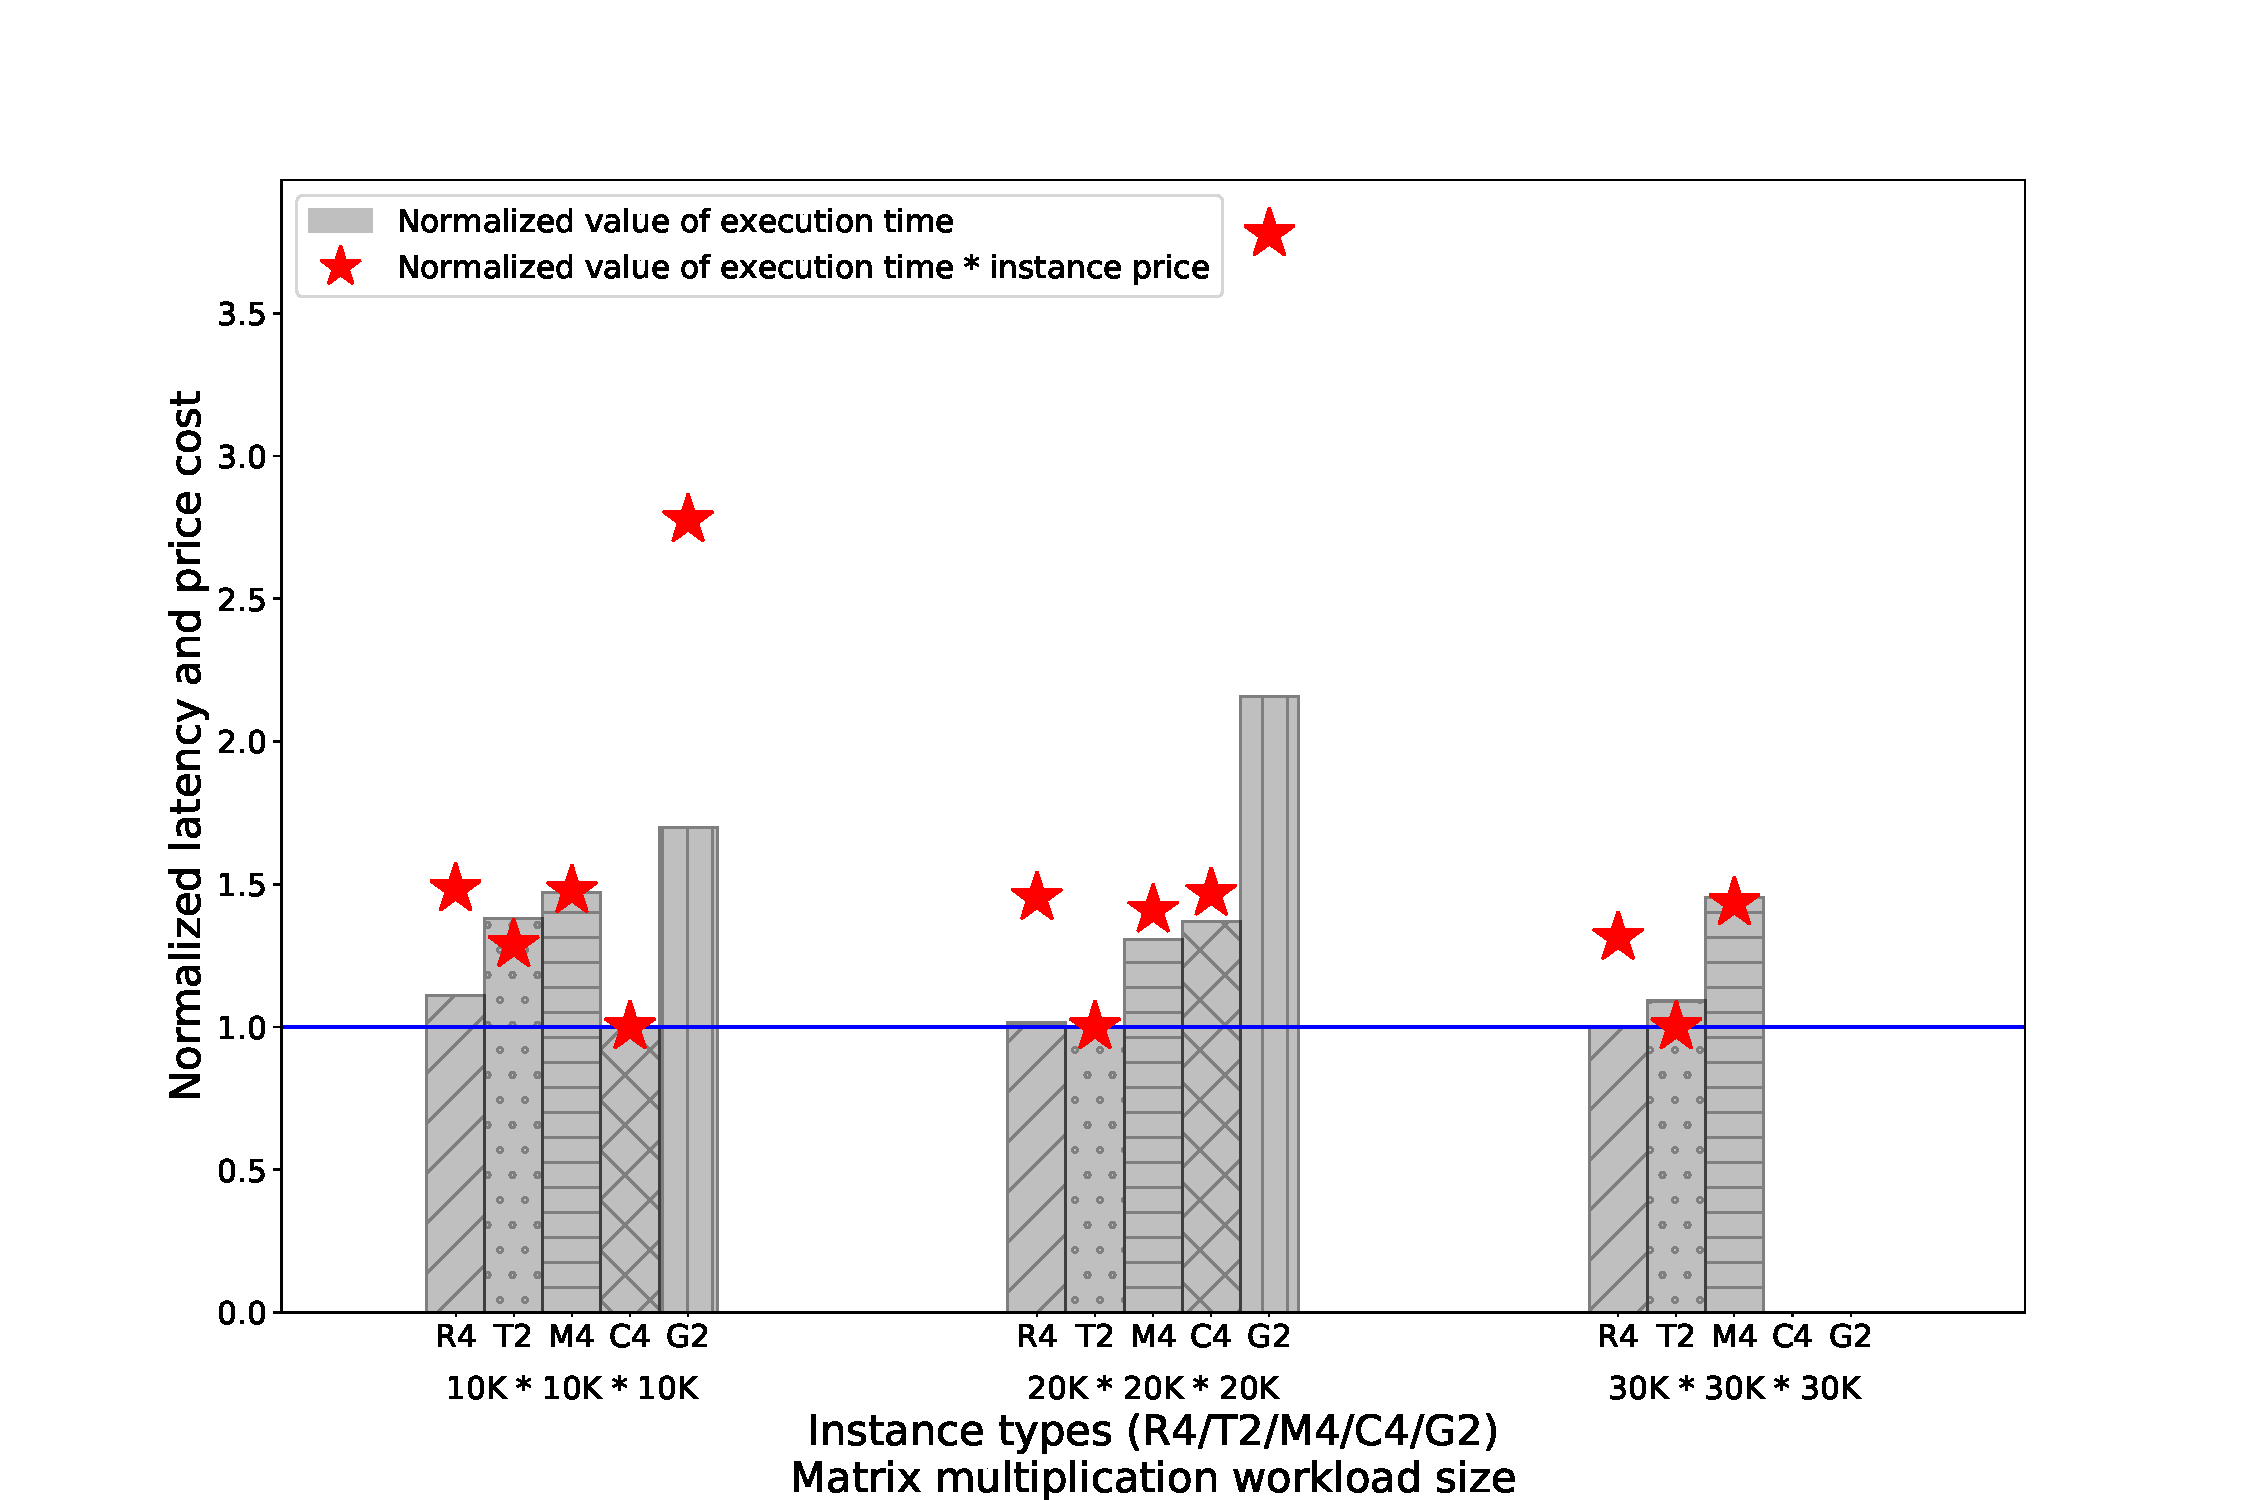
\includegraphics[width=4.5cm,height=4.5cm]{figures/instance-2xl-compare.pdf}}\hfil\hfil\hfil\hfil\hfil\hfil\hfil\hfil\hfil\hfil\subfloat[Performance of different matrix shapes]{\label{fig:different-matrix-shapes}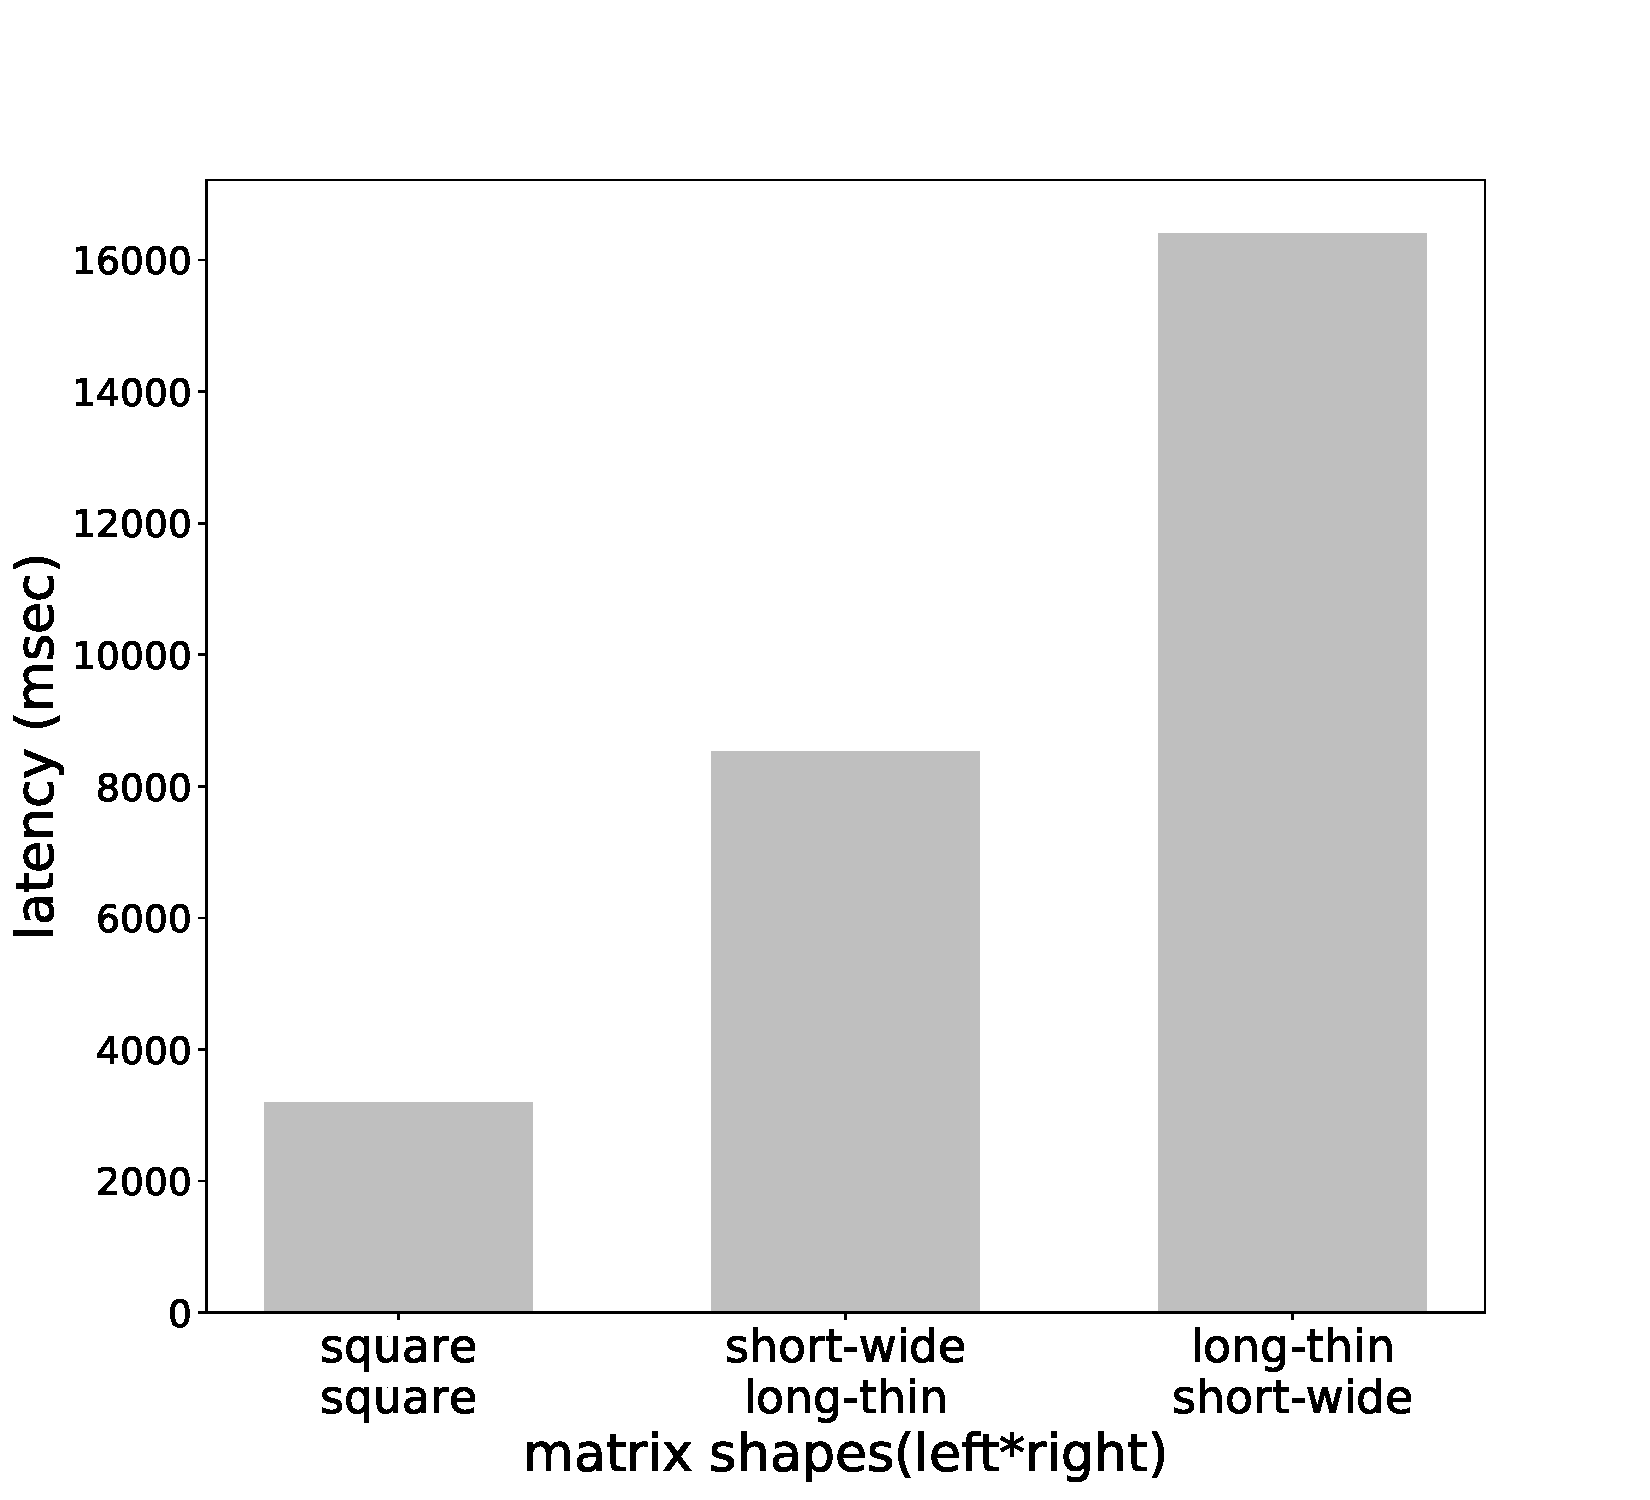
\includegraphics[width=4cm, height=4.5cm]{figures/matrix-multiplication-different-shape.pdf}}
  \caption{\label{fig:instance-blocks-sizes-compare}. The normalized value of latency with respect to different instance types and input matrix shapes - the lower, the better.}
\end{figure}

Despite of the importance of the matrix multiplication when running machine learning tasks, performance analysis and modeling in a distributed cloud computing environment are not thoroughly conducted yet. Few works focused on predicting data mining algorithm performance on a cloud computing environment - Ernest~\cite{ernest}, CherryPick~\cite{cherrypick}, and PARIS~\cite{paris}. The proposed methods rely on a scale-based sampling method to estimate the latency to complete original large input size, and they show poor accuracy when predicting distributed matrix multiplication task running time as they fail to capture the nature of distributed matrix computation. Performance modeling and prediction on a single machine with multiple cores are well studied in literature with hardware optimized libraries, such as OpenBLAS, but previous works generally do not consider network and IO overhead that can be additional significant overhead in a distributed cloud computing environment.

In this paper, we propose MPC (\textbf{M}atrix Multiplication \textbf{P}erformance Predictor for \textbf{C}loud Computing) to provide accurate latency prediction while performing multiplication of arbitrary shape and size of matrices on diverse cloud computing resources. MPC profiles the latency to perform multiplication on two unit-block matrices on diverse cloud computing resources. In order to represent the profiled unit-block latency results, MPC builds a model with XXXX followed by bayesian optimization to find the optimal hyper parameters to minimize the modeling error. In the step of prediction of arbitrary size matrix multiplication, MPC proposes to disassemble the input matrices into blocks that worker nodes can operate, and the latency to multiply each block matrix is made by using the model built from the unit-block matrices. MPC eventually stitches the blocks to conjecture the overall task completion time.

% summarize the result
% itemize the contributions

\section{Matrix Multiplication on a Distributed Computing Environment}\label{sec:distributed-matrix-computation}
% explain how the matrix computation happens in spark - mention the step of shuffle, compute, reduce
% How block matrix multiplication happens with the overhead (shuffle, compute, reduce)
Optimization of distributed matrix multiplication is well studied in the literature. In the HPC community, many works focused on minimizing communication cost using MPI model. Representative works include SUMMA~\cite{summa} and CARMA~\cite{carma}. Despite of the performance optimality of the methods, they have limitations regarding the programmability, scalability, and robustness comparing to general purpose big-data analytics systems, such as Spark~\cite{spark} and Hadoop~\cite{hadoop}, especially on a shared cloud computing environment.

0Apache Spark is an open source big-data analytics platform. The primary abstraction in Spark is Resilient Distributed Dataset(RDD), which represents a read-only collection of objects partitioned across a set of machines. Spark manages large-scale data using partitions that helps parallelize distributed data processing while guaranteeing the fault-tolerance with lineage and task execution optimization with lazy evaluation~\cite{spark}.

In Spark, matrix-related linear algebraic operations are supported in the MLLib library~\cite{spark-mm} with various matrix partitioning heuristics (row-, column-, and block-based) and a set of distributed operation APIs on the matrix. To multiply two matrices, Spark MLLib automatically identifies the optimal way of task distribution based on the input matrix partitioning scheme and uses Scala Breeze library to execute multiplication. Let us give an example of multiplying two matrices, $C = A \times B$. If $A$ is row-partitioned and $B$ is column-partitioned, the cartesian product is performed for each row block of $A$ and column block of $B$. If both $A$ and $B$ are block-partitioned, the block dimension of result matrix, $C$, is decided by considering the number of workers and input block dimensions. A work node that is responsible for each resulting block fetches all the necessary blocks from $A$ and $B$ to execute multiply operation locally.

\begin{figure}
  \centering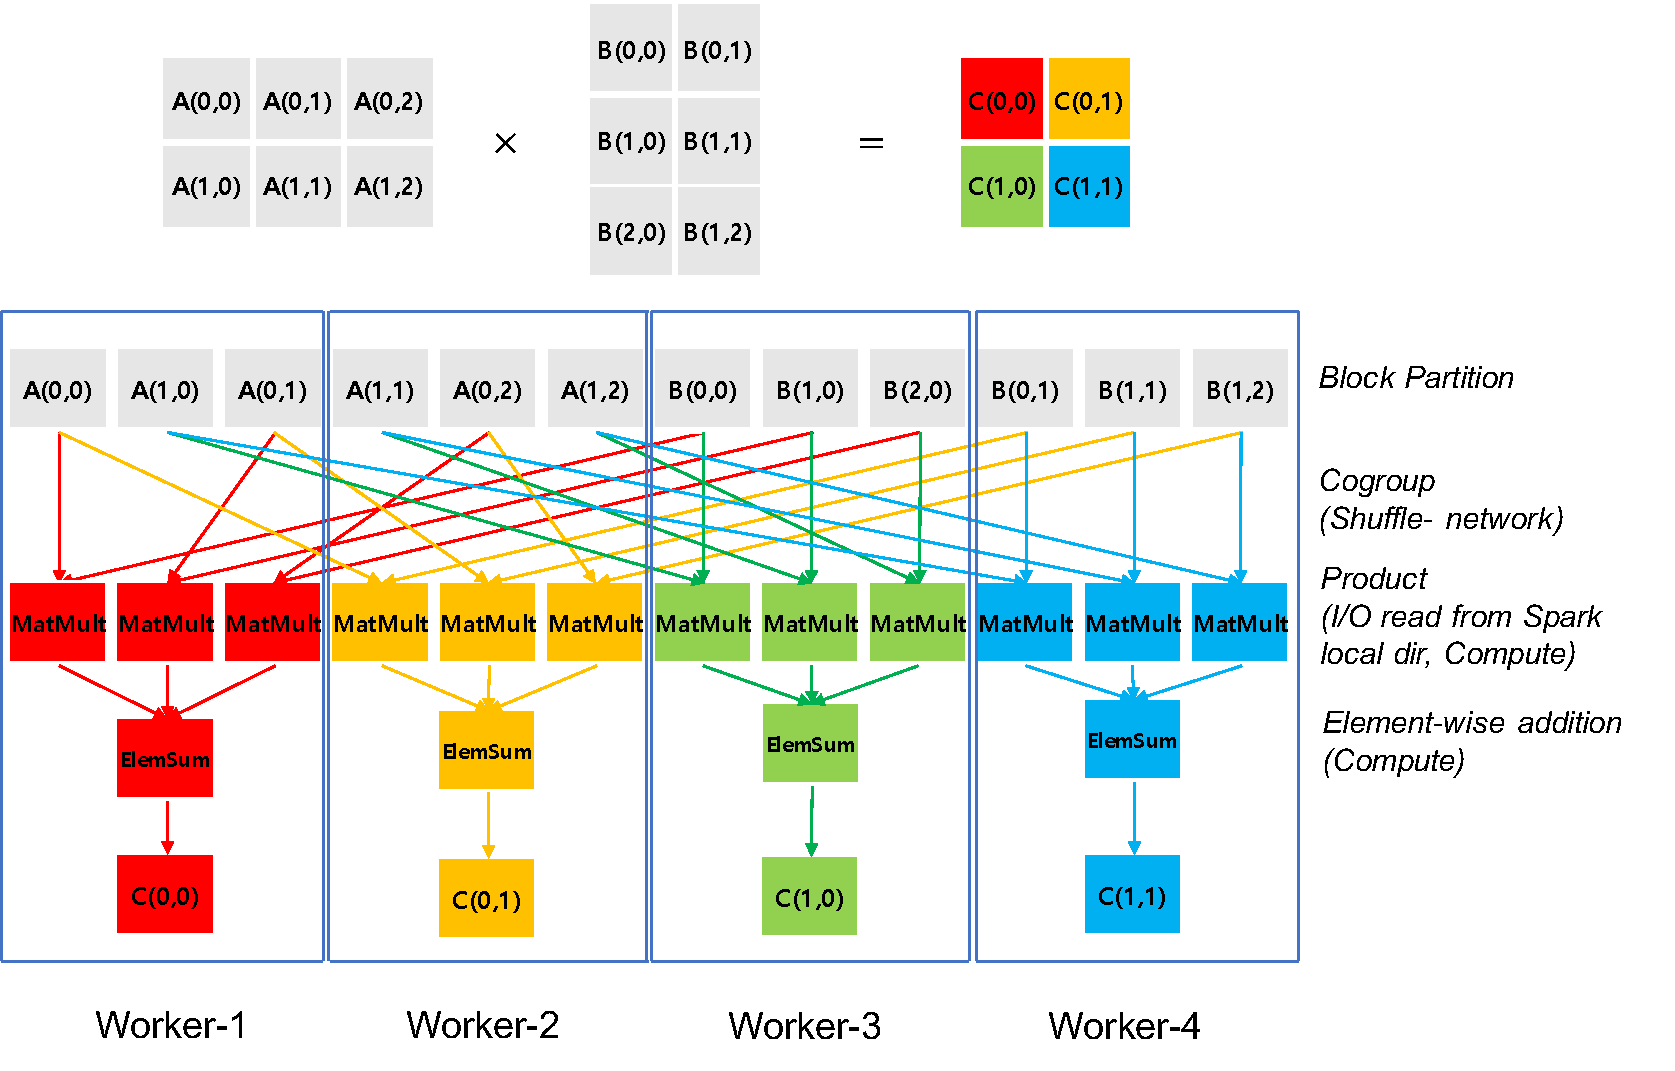
\includegraphics[width=0.45\textwidth]{figures/matmult-overhead-non-square.pdf}\caption{Block-based distributed matrix multiplication and its overhead in each step. Network, IO, and CPU are principal resources for the execution.}\label{fig:matmul-with-overhead}
\end{figure}
Figure~\ref{fig:matmul-with-overhead} shows an example of block-based matrix multiplication. A left matrix, $A$, is block-partitioned by $2 \times 3$, a right matrix, $B$, is partitioned by $3 \times 2$, and the result matrix, $C$, is partitioned by $2 \times 2$. In Spark, a \textit{cogroup} operation by the result matrix block index allows a worker node that is responsible for a result block to collect necessary left and right matrix blocks. During \textit{cogroup} operation, network overhead is dominant. After collecting all necessary blocks, each worker node performs a product operation followed by an element-wise addition. In the step, I/O overhead to read the fetched blocks from a \textit{local.dir} location and compute overhead dominates.

\subsection{Distributed Matrix Multiplication Overhead Modeling}\label{sec:overhead-modeling}
Dense matrix multiplication is widely known as a CPU intensive task, but other resource overheads become non-negligible when it is executed on a large-scale distributed computing environment, such as Spark. To qualitatively understand the characteristics of a distributed matrix multiplication task, we summarize overheads when a task is executed on Apache Spark. Let us assume the number of rows of a left matrix as $N$, the number of columns of a left matrix (or the number of rows of a right matrix) as $K$, and the number of columns of a right matrix as $M$. Accordingly, the result matrix size is $N \times M$. Left, right, and result matrices are block-partitioned whose partition size is expressed in the lowercase letter ($n$, $k$, and $m$, where $N \geq n$, $M \geq m$, and $K \geq k$). 

\textbf{Shuffle}: A worker node that is responsible for computing an output matrix block of size $n \times m$ has to fetch blocks from left and right matrices with the size of $n \times K$ and $K \times m$, respectively. If a worker node does not contain required blocks locally, it has to fetch them from remote machines that incur network overhead. Assuming uniform block distribution among workers, the network overhead in the shuffle phase can be expressed as Equation~\ref{eq:shuffle-overhead}.
\begin{equation}\label{eq:shuffle-overhead}
  BlockFetchOverhead_{n \times m} \propto \sum\limits_{i=1}^{\frac{K}{k}} n \times k + k \times m
\end{equation}

\textbf{Compute}: After a shuffle step completes, a worker node performs multiplication of fetched blocks followed by element-wise addition. In order to perform multiplication, the blocks have to be read from a Spark local directory (\textit{spark.local.dir} configuration) that is generally set as a disk. Thus, the IO read overhead is same as the shuffle overhead and expressed as Equation~\ref{eq:shuffle-overhead}.

After loading the input matrix blocks, each worker node executes a multiplication task whose overhead is expressed as Equation~\ref{eq:compute-overhead}.
\begin{equation}\label{eq:compute-overhead}
  ComputeOverhead_{n \times m} \propto \sum\limits_{i=1}^{\frac{K}{k}} n \times k \times m
\end{equation}

In the element-wise addition step, the number of sum operation of each cell is proportional to $k$, and the size of each output block is $n \times m$.

\section{MPC : Matrix Multiplication Performance Prediction}\label{sec:mpc-structure}
MPC aims to predict the latency to complete multiplication of dense matrices that might have different size and shape. As the matrix multiplication is a core kernel method for various machine learning algorithm for big-data analytics, we target to predict the performance on various cloud computing resources where many recent big-data systems are deployed.

\begin{figure}
  \centering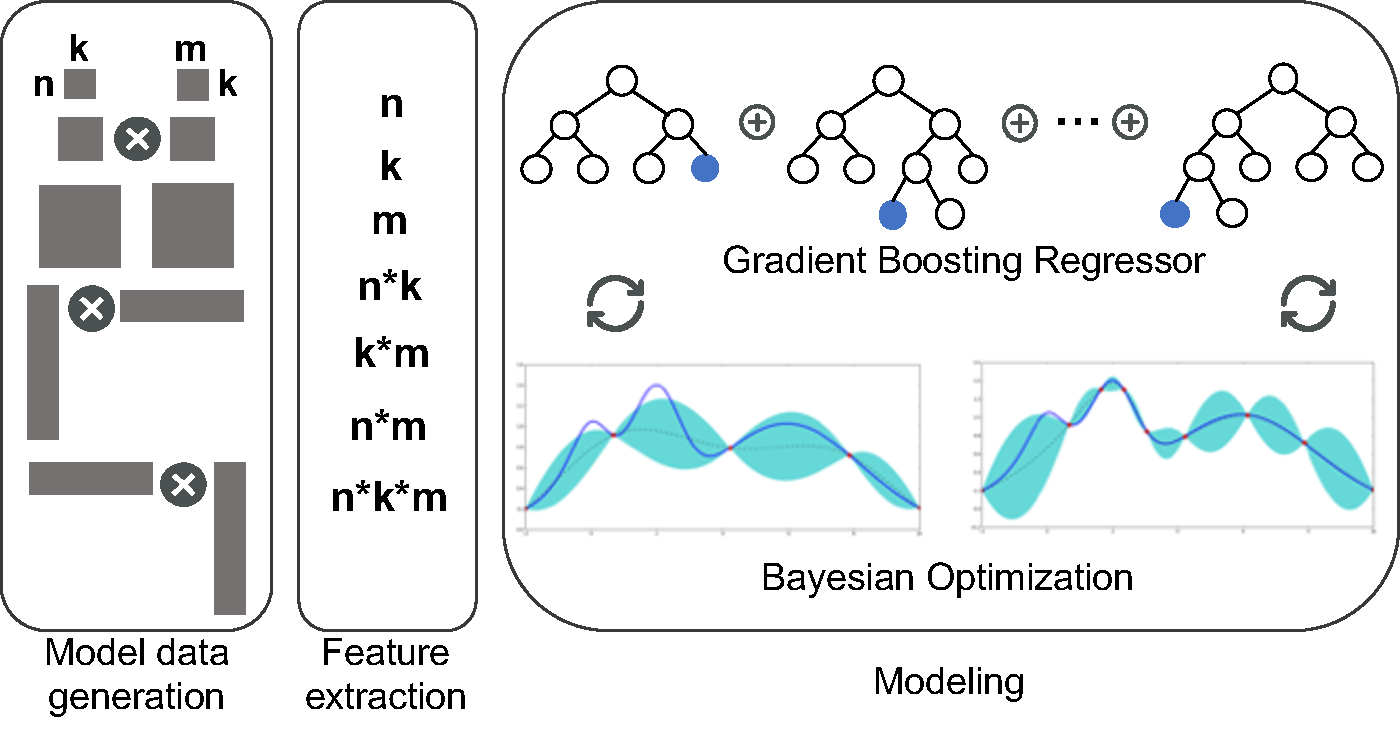
\includegraphics[width=0.5\textwidth]{figures/mpc-architecture.pdf}\caption{Architecture of MPC to predict various matrix multiplication performance}\label{fig:mpc-architecture}
\end{figure}

The operation step of MPC is shown in Figure~\ref{fig:mpc-architecture} that is composed of train dataset generation, feature extraction, and modeling. In the modeling step, we iteratively apply bayesian optimization~\cite{bayesian-optimization} to find the optimally working hyper parameters of the chosen algorithm.

\subsection{Train Data Generation}\label{sec:train-data}
In the train data generation step, MPC performs offline profiling of various types and sizes of matrix multiplication to build a model to predict latency of arbitrary input dataset. A matrix multiplication task can be broadly grouped into square $\times$ square, long-thin $\times$ short-wide, and short-wide $\times$ long-thin matrices. To cover all the shapes and various sizes, MPC profiles the latency of synthetically generated left and right matrices. In the latency measurement, MPC utilizes Apache Spark WebUI REST API that provides various execution metrics in the JSON format.

To consider various cloud computing instances with distinct capacity, MPC adopts OpenBLAS to conduct computation on CPU and NVBLAS to conduct computation on instances that equip GPU devices. To allow Spark to interact with the hardware-optimized linear algebra libraries, we use netlib-java as proposed in~\cite{fatman-littleboy}.

\subsection{Feature Extraction}\label{sec:features}
As shown in Section~\ref{sec:overhead-modeling}, overheads of matrix multiplication in a distributed computing environments encompass various sources of resources. In order to account for such diverse overheads, MPC proposes to utilize the dimension of input matrix blocks and the products, namely $n$, $m$, $k$, $n \times m$, $n \times k$, $k \times m$, and $n \times k \times m$, as features to model the performance. With $n \times m$ term, we can consider the size of output matrix, $n \times k$ and $k \times m$ terms represent the size of left and right matrix blocks size that impacts network and IO disk overhead. The $n \times k \times m$ term represents the total number of multiply operations.

Different from MPC, previous works that focus on predicting the performance of data mining tasks on cloud computing resources used a scale-based sampling mechanism as an input feature for prediction~\cite{ernest, cherrypick, paris}. They generally apply sampling at the input dataset by selecting very small portion and measure performance using the subset of the dataset. Using the outcomes from the sample dataset, different algorithms apply distinct predictive algorithms, such as non negative linear equation (Ernest~\cite{ernest}), bayesian optimization (Cherrypick~\cite{cherrypick}), and random forest (PARIS~\cite{paris}), to make prediction. However, the scale-based sampling mechanism cannot capture the complex nature of distributed matrix multiplication, and it considers either $n$ or $m$ based on the sampling method. In the evaluation section, we demonstrate the superior performance of MPC due to the rich set of features.

\subsection{Modeling}\label{sec:modeling}
In the modeling step, MPC builds a model to represent the performance of multiplying various matrices. This step is composed of model build and hyper parameter search; MPC utilizes Gradient Boosting~\cite{gradient-boosting} regressor for model build step and Bayesian Optimization~\cite{bayesian-optimization} to find the optimal parameters to run GB method.

Gradient Boosting~\cite{gradient-boosting} is a flexible non-parametric statistical learning approach for classification and regression. The main idea of GB is combining many weak learners that are generally applicable only to simple linear relations incrementally to model complex and non-linear interactions among features. A GB model is fitted in a forward stage-wise pattern; at each stage, a new weak learner model is fit to the residual of the current model, and it focuses more on correcting errors from the previous iterations. Different from a similar decision tree method, GB is known to be robust to overfitting by ensembling many weak learners~\cite{random-forest}.

When building a predictive model, properly setting model parameters is crucial to improving the quality of prediction. Many heuristics to search for the best performing hyper parameters are proposed, such as random walk, grid-based search, or using a statistical inference method. Among them, MPC utilizes a statistical inference method based on the bayesian model~\cite{bayesian-optimization}. The bayesian optimization method searches for a set of next configuration values that is likely to improve model quality or to decrease uncertainty. It is a non-parametric black box approach that estimates an objective function (i.e., the complete performance measure from all combinations of parameters) using a stochastic process, such as Gaussian process. In predicting the objective function, bayesian optimization uses all of the information available from previous runs ($prior$), and the objective function model is updated ($posterior$) after new experiments are conducted ($likelihood$). 

\section{Evaluation}{\label{sec:eval}}
In this section, we evaluate the performance of MPC thoroughly from the perspective of input matrix variability and cloud instance type diversity. Applying gradient boosting algorithm with the proposed features outperforms linear regressor by showing XY\% more prediction accuracy. Furthermore, by applying bayesian optimization to select optimal hyper-parameters of gradient boosting, we could improve the accuracy about XY\%. Evaluation of MPC with various cloud instance types demonstrates the effectiveness of MPC on a cloud computing environment. Finally, comparing MPC with Ernest~\cite{ernest}, the state-of-the-art machine learning performance predictor on cloud, shows that MPC has about XY\% more accuracy in predicting matrix multiplication latency.

\subsection{Setup}
To make diverse matrix multiplication scenarios for training and evaluation, we varied the number of rows and columns of left and right matrices from 128 to 800,000. Within the range, we generate XYZ(number of dataset) cases of square $\times$ square, long-thin $\times$ short-wide, and short-wide $\times$ long-thin matrices\footnote{test input cases - bit.ly/xyz}. The matrix multiplication is performed with Apache Spark and MLLib library with a version of 2.2.0. Multiplication of each matrix size is executed five times, and the average value is used to represent the latency for a task. A spark cluster is deployed to AWS EC2 by using \textit{spark-ec2} library\footnote{https://github.com/kmu-leeky/spark-ec2} with four \textit{R4.2xlarge} instances, unless otherwise stated. Each EC2 instance has hardware-optimized linear algebra library installed, namely NVBlas for a GPU instance (\textit{g2.2xlarge}) and OpenBlas for other instances. For matrix multiplication modeling and evaluation, we use \textit{scikit-learn} 0.18.1 with \textit{Python} 2.7.12. To evaluate the accuracy of prediction models, we use \textit{coefficient of determination} ($R^2$) as a metric. The metric is calculated as Equation~\ref{eq:cod}, and it measures how much the predicted outcome ($\hat{y_i}$) resembles the measured value ($y_i$). The maximum value of the metric is $1.0$ that says the model predicts without an error (the larger, the better).

\begin{equation}\label{eq:cod}
  R^2 = \frac{\sum\limits_{i} (\hat{y_i}-\overline{y})^2}{\sum\limits_{i} (y_i-\overline{y})^2}
\end{equation}


\subsection{MPC Performance Evaluation}
\subsubsection{feature importance} MPC proposes to use various combinations of left and right matrix block sizes as features to model complex mechanism of distributed matrix multiplication. To assess the impact of features in the model, we show the relative importance of features that are calculated by counting the number of times a feature is selected for splitting where each split is weighted by the improved performance~\cite{gb-feature-importance} in Figure~\ref{fig:feature-importance} gray bars. \emph{GradientBoostingRegressor} method is performed 100 times, and the average importance value is shown with the minimum and maximum value in the error bar. The total number of multiply operation ($lr \times lc \times rc$) term is the dominant feature (0.30) as people generally expect. However, a feature that represents the output matrix size ($lr \times rc$) and shuffle overhead ($lr \times lc + rr \times rc$) are also dominant factors, $0.25$ and $0.20$, respectively, and this observation corresponds to Figure~\ref{fig:different-matrix-shapes} that shows the latency might differ for the same matrix size with different shape and output size, e.g., long-thin $\times$ short-wide versus short-wide $\times$ long-thin. To quantitatively analyze the impact of each feature to the model accuracy, we show the coefficient of determination value in the secondary vertical axis. From the most important feature, we cumulatively add a next important feature (in the x-axis) and build a model. The best model accuracy is achieved with three most important features (the number of multiply operations, output matrix size, and the amount of shuffle overhead).

\begin{figure}
  \centering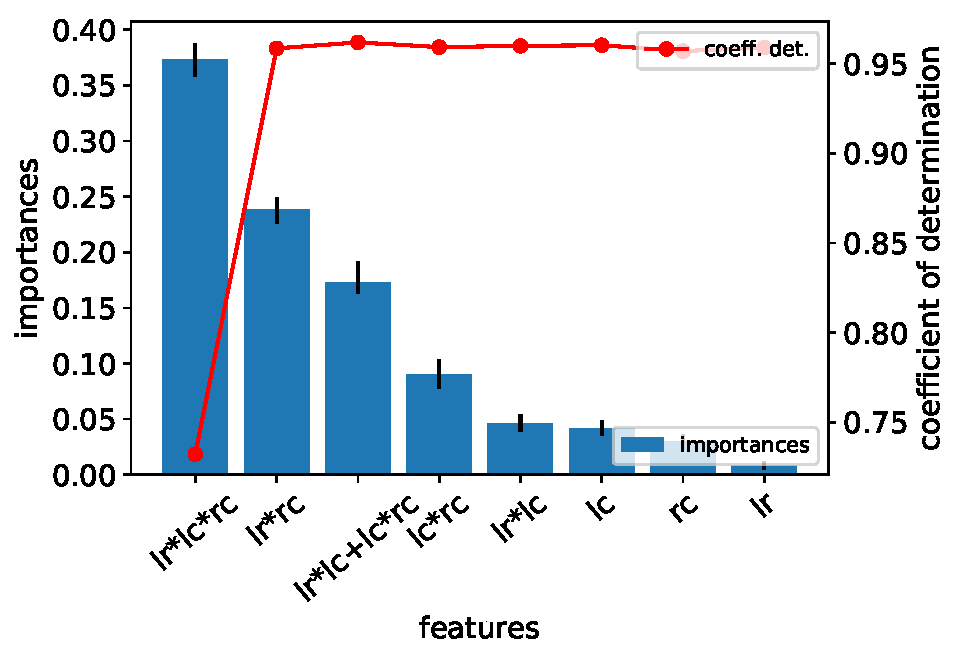
\includegraphics[width=0.45\textwidth]{figures/feature-importance.pdf}\caption{The relative importance of features and the impact to the model accuracy. The number of multiply operations, output matrix size, and  the shuffle overhead are the three most important features.}\label{fig:feature-importance}
\end{figure}

\subsubsection{effectiveness of bayesian optimization} MPC uses bayesian optimization to find the optimal hyper parameters to build a model. To quantitatively analyze influence from the optimization step, we show three hyper parameters and the $R^2$ value in Table~\ref{table:bo-performance}. In the experiment, we use \textit{BayesianOptimization} library from \textit{bayes\_opt} package in Python. During optimization, we split the input dataset as a train and test set with the 10-fold cross validation method, and 40 iterations with different hyper parameters are evaluated. Comparing to default parameters of \textit{GradientBoostingRegressor}, the optimization step changes the parameters in the direction of increasing accuracy, i.e., more number of regression trees (n\_estimators), while controlling overfitting, i.e., avoid modeling a case specific to a particular sample (min\_samples\_split). In the final row, we can see the accuracy of the model measured as a coefficient of determination increases slightly from $0.9578$ to $0.9681$.

\begin{table}
  \centering
  \begin{tabular}{|C{2.2cm}|C{1.5cm}|C{1.5cm}|}
  \hline
  &default&bayesian optimization\\
  \hline
  n\_estimators&100&235\\
  \hline
  min\_samples\_split&2&16\\
  \hline
  max\_features&8&6\\
  \hline
  performance ($R^2$)&0.9578&0.9681\\
  \hline
  \end{tabular}
  \caption{\label{table:bo-performance}Paramters suggested by optimization module and the improved performance}
\end{table}

\subsubsection{prediction algorithm comparison}
To predict the execution time of matrix multiplication of arbitrary sizes and shapes, various machine learning algorithms can be applied with features that are proposed in this paper. Among the algorithms, we compare decision tree regression variant algorithms and a linear regrssion variant method. For the decision tree variants, we compare gradient boosting regressor that is introduced in Section~\ref{sec:modeling} and random forest~\cite{random-forest}. Different from gradient boosting, random forest regressor builds multiple regressor trees by randomly selecting features and samples. Both gradient boosting and random forest regressors represent the non-linear character of input data while preventing over-fitting by combining outcomes from many weak learners. As a linear regression variant method, we adopt non-negative least squares (NNLS) regressor. In predicting latency, the non-negativity constraint should be imposed to avoid the latency being less than zero, and NNLS finds the optimal linear model that minimizes the prediction error.

\begin{figure}[t]
	\centering
	\subfloat[performance w.r.t instances ]{\label{fig:gbm-r2-score}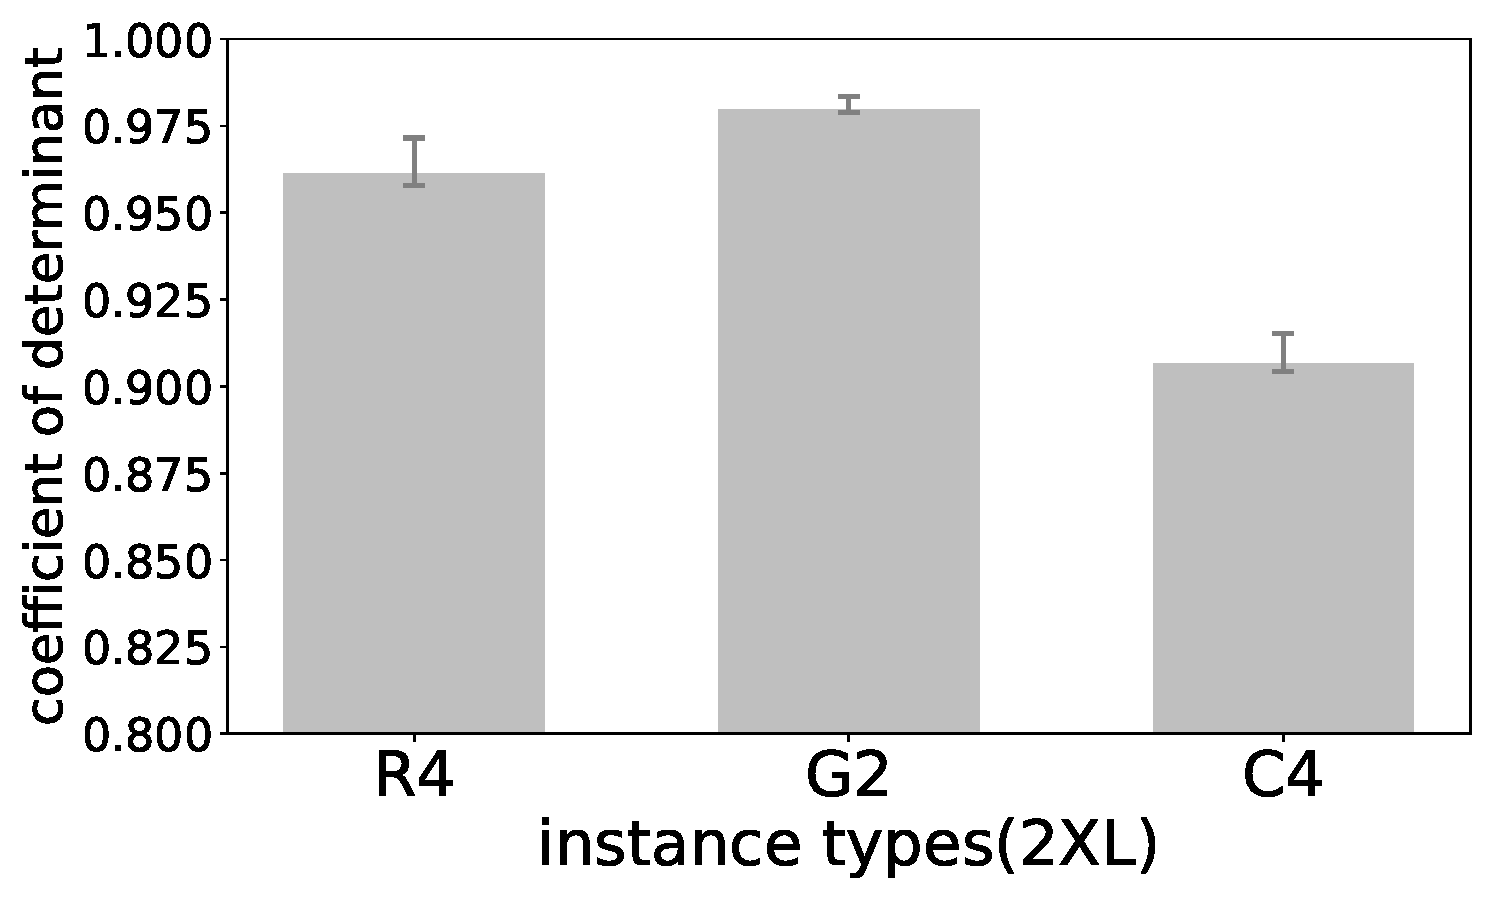
\includegraphics[width=0.4\textwidth]{figures/compare-instances-gbm-r2.pdf}}\\ 
	\subfloat[Measured/Predicted]{\label{fig:gbm-measured-predicted-ticks}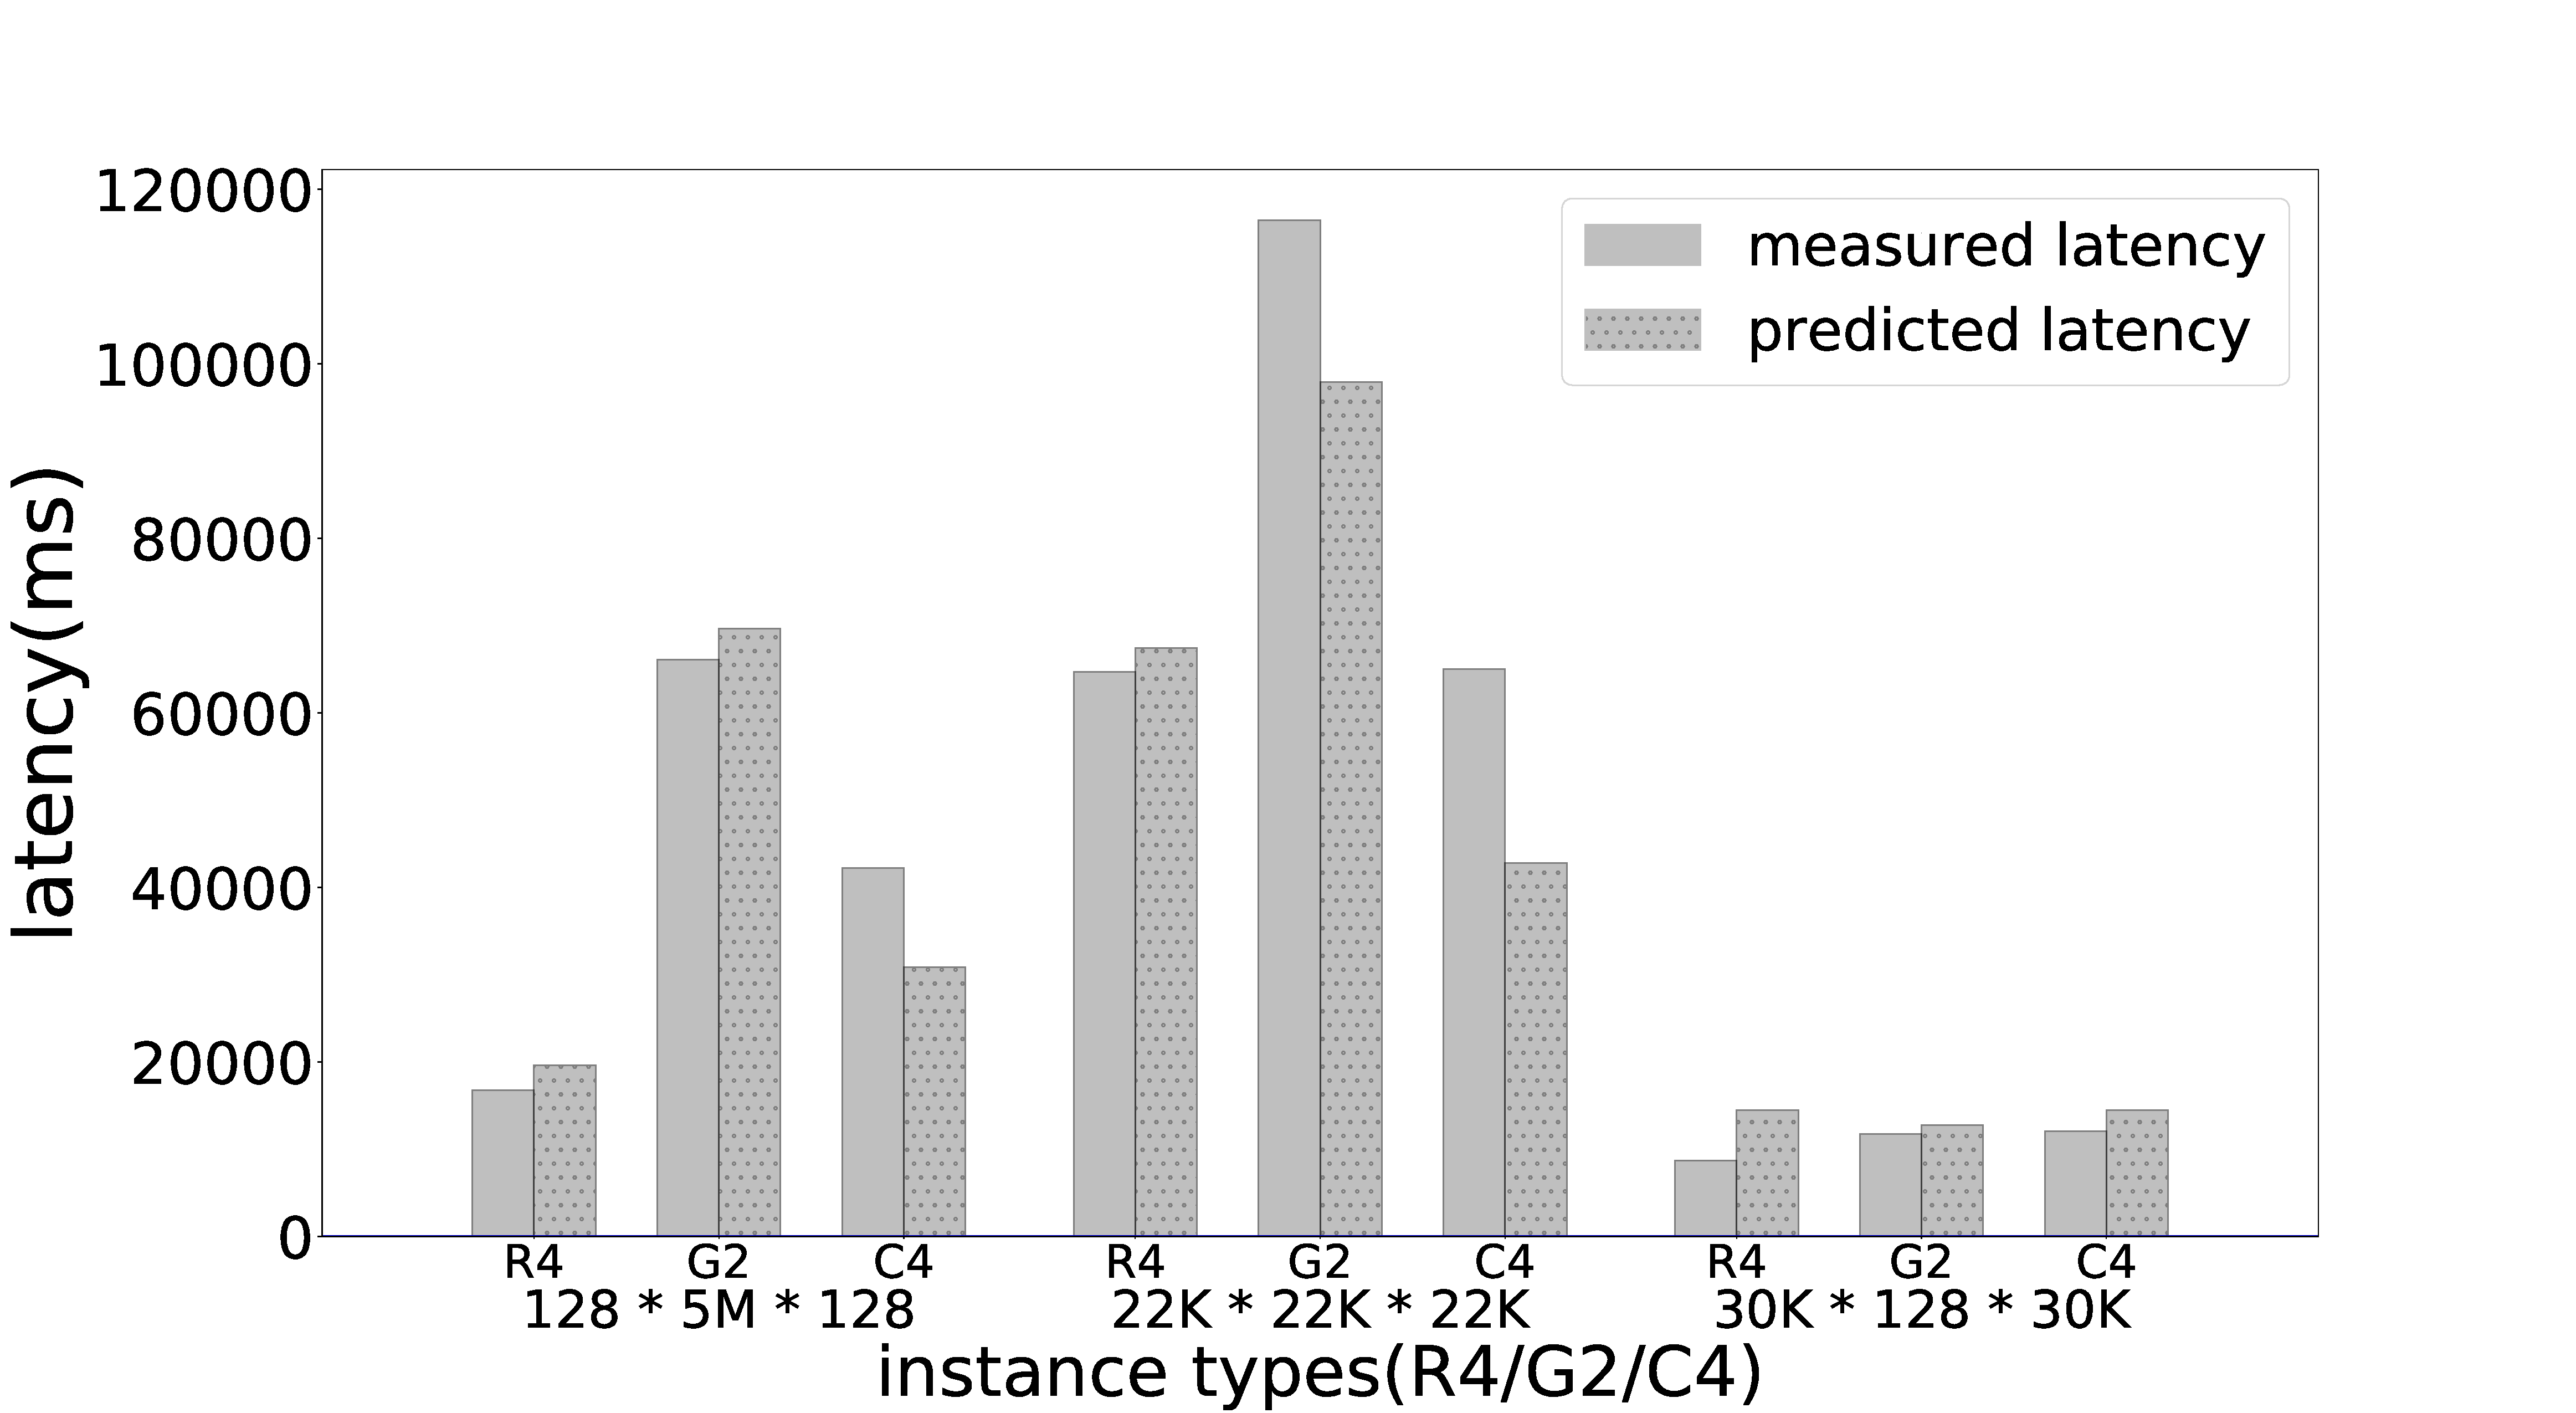
\includegraphics[width=0.5\textwidth]{figures/GBM-measured-predicted-ticks.pdf}} \hfil 
	\caption{\label{fig:gbm-comparison}. GBM performance}
\end{figure}

Figure~\ref{fig:r2-comparison} shows the prediction accuracy of three different algorithms. For each algorithm, we use the train dataset and features that are presented in Section~\ref{sec:mpc-structure}. 10-fold cross validation is performed 100 times, and the average value is plotted with the minimum and maximum value in the error bars. The gradient boosting regressor shows the best accuracy with the $R^2$ value of $0.968$, followed by random forest regressor and NNLS with the $R^2$ of $0.955$ and $0.869$, respectively. From the figure, we can see that the linear equation cannot capture the non-linear interactions among proposed features in this paper. Figure~\ref{fig:gbm-measured-predicted} (gradient boosting regressor) and \ref{fig:nnls-measured-predicted} (NNLS) show the measured latency and predicted latency in the x and y axis, respectively. The dotted line means the prediction with no error (slope of one), and scattered points close to the line are accurate predictions. From the figures, we can confirm that the gradient boosting regressor provides better accuracy in the latency prediction.

\begin{figure}[t]
  \centering
  \subfloat[algorithms performance comparison]{\label{fig:r2-comparison}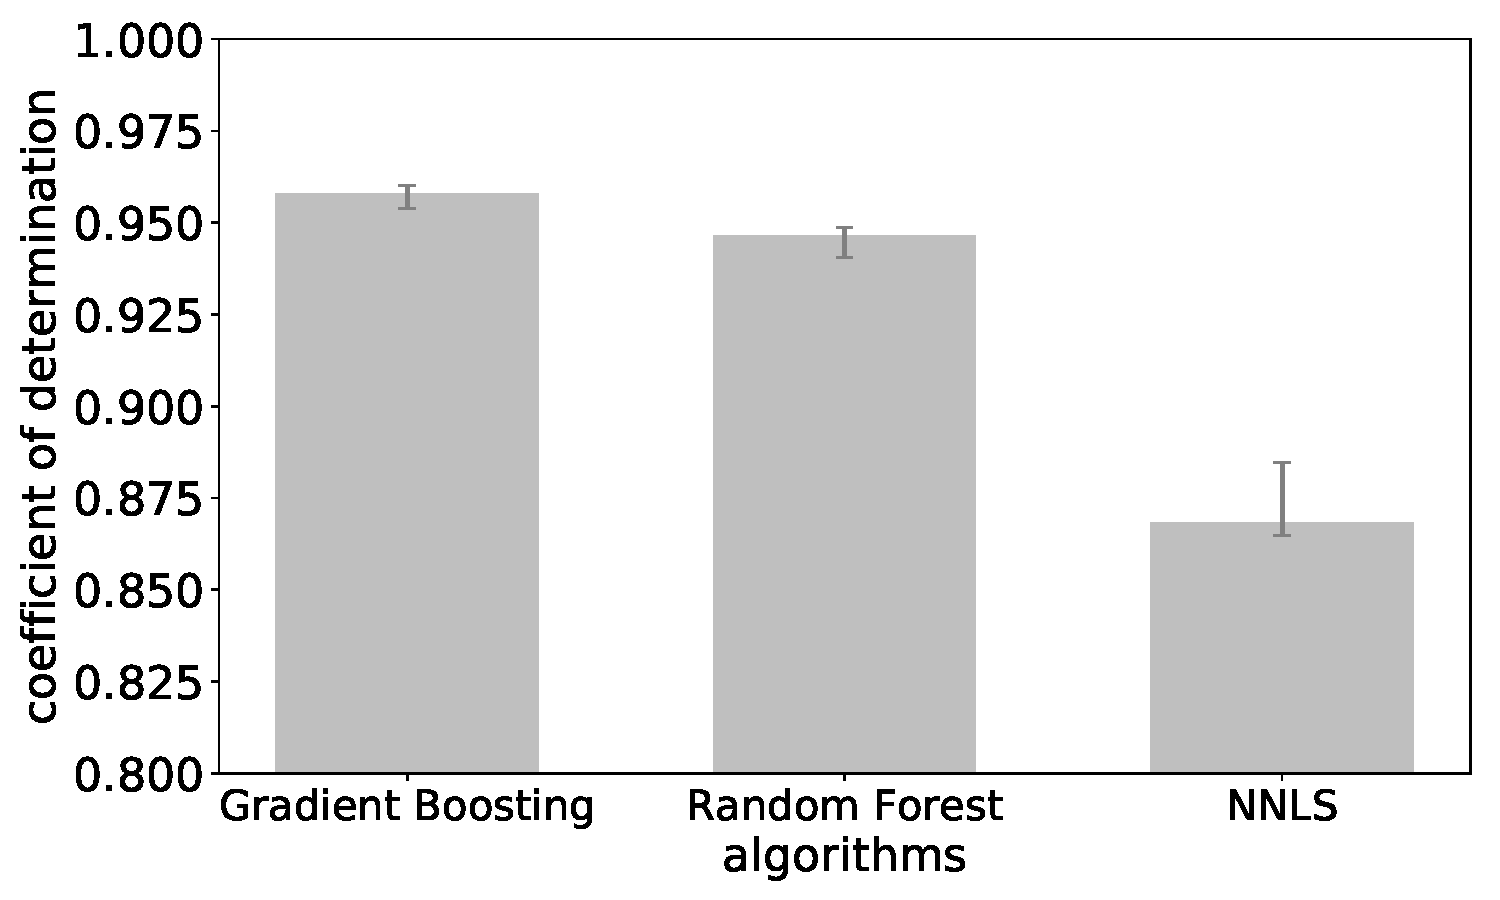
\includegraphics[width=0.4\textwidth]{figures/compare-algorithms.pdf}}\\ 
  \subfloat[GBM]{\label{fig:gbm-measured-predicted}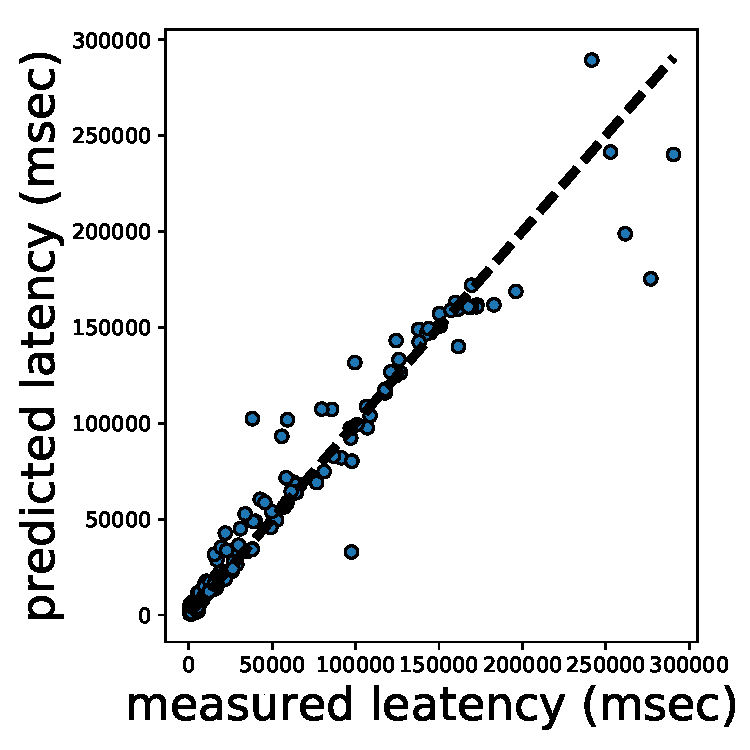
\includegraphics[width=0.23\textwidth]{figures/gbm-measured-predicted.pdf}} \hfil \subfloat[NNLS]{\label{fig:nnls-measured-predicted}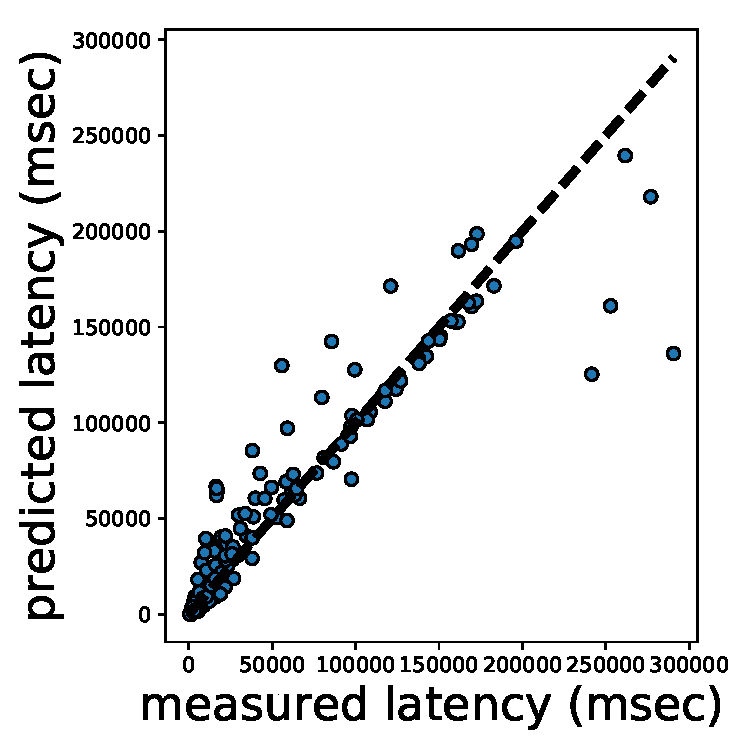
\includegraphics[width=0.23\textwidth]{figures/nnls-measured-predicted.pdf}}
  \caption{\label{fig:algorithm-comparison}. Performance comparison}
\end{figure}



% prediction on cloud computing instances
% two figures - using GB, R^2 is consistent for C4, R4, G2
% - three representative matrices, the latency becomes different, we can also mention the price

\subsection{Comparison with Ernest}
% choose three cases with the largest size. run the test see the result.


\begin{figure}[t]
	\centering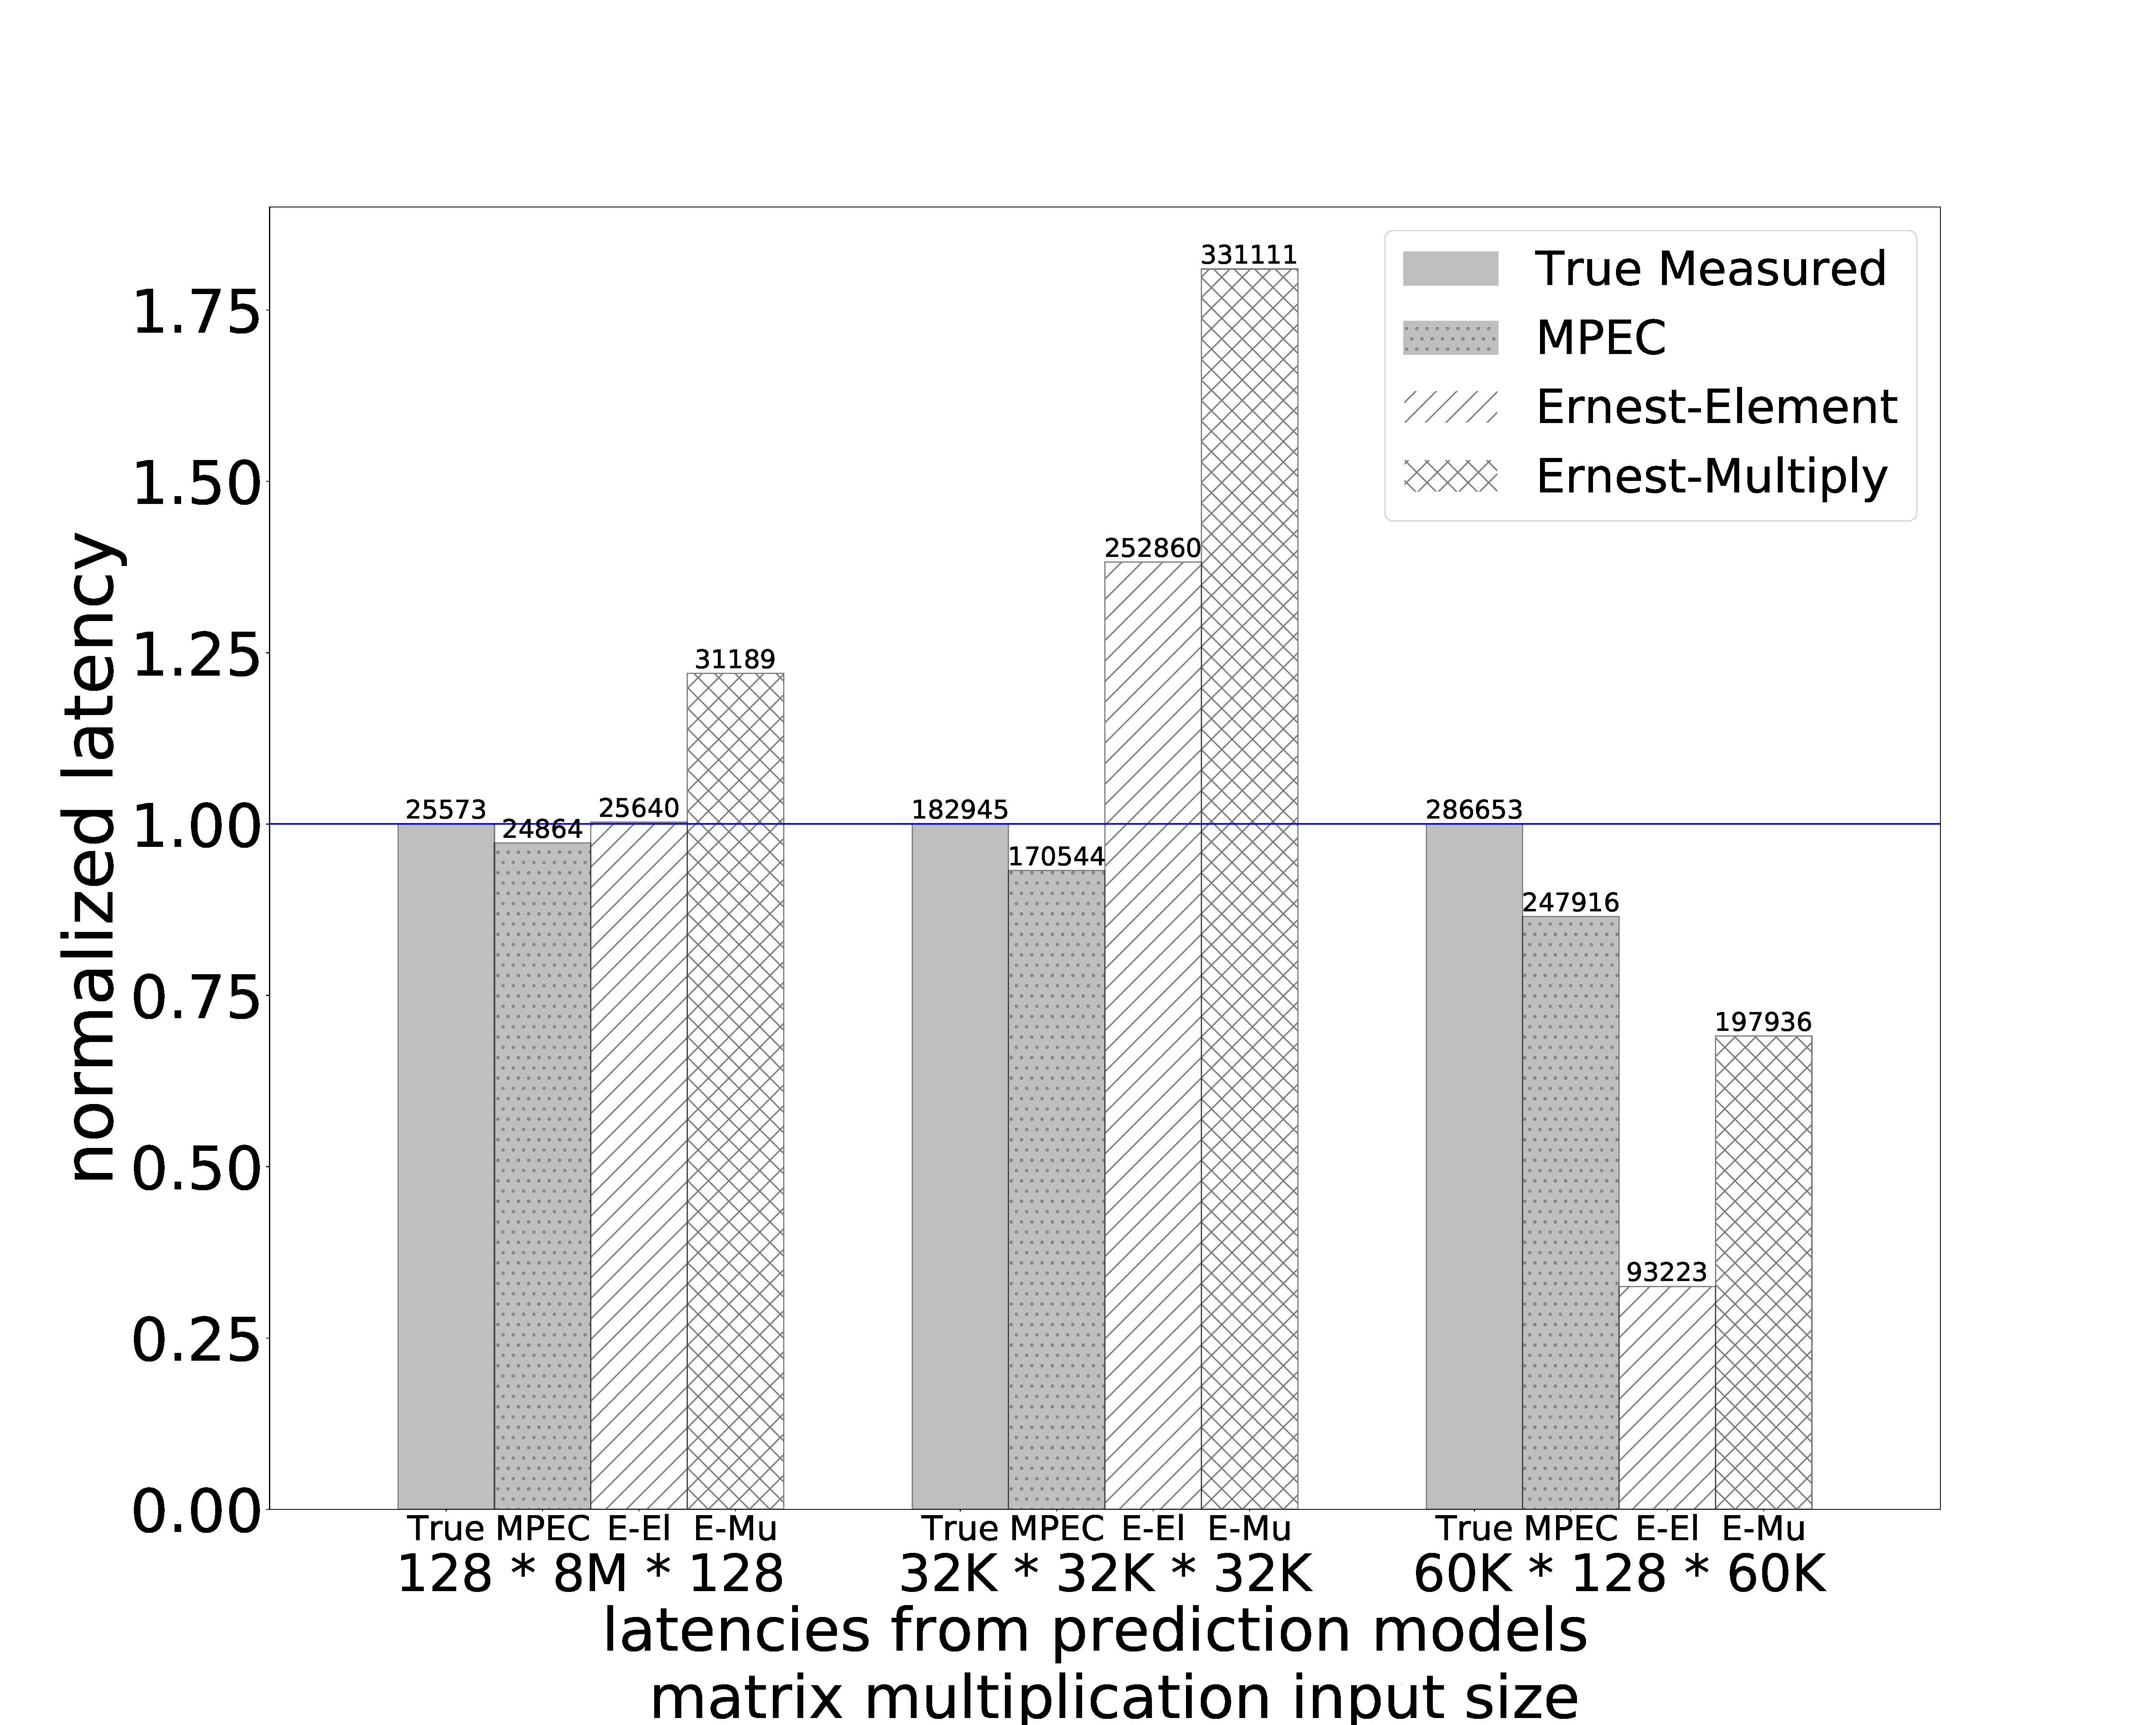
\includegraphics[width=0.4\textwidth]{figures/MPC-Ernest-compare.pdf}\caption{Comparsion with MPC}\label{fig:mpc-ernest}
\end{figure}

\section{Related Work}\label{sec:relatedwork}
\textbf{Big-data workload performance estimation on cloud}: In a cloud computing environment, there are a large number of instance types that have unique hardware configurations, and few works propose a method to build an optimal environment to run big-data analytics workloads. Ernest~\cite{ernest} proposes a method to predict performance of running arbitrary data mining algorithms with different number of resources on cloud. The proposed algorithm is composed of two parts, an experiment design step to select candidates of input data set to perform profiling and a prediction step to calculate the expected latency with a different number of resources. PARIS~\cite{paris} takes a hybrid online/offline approach, using a random forest model to predict application performance on various VM configurations based on features such as CPU utilization obtained from profiling. Cherrypick~\cite{cherrypick} proposes to use bayesian optimization to select instance type candidates to perform off-line profiling to predict performance on various cloud instance types. The works rely on a sampling method for a given input dataset, and the profiled result is not reusable for other input datasets. Furthermore, they focus on predicting high-level machine learning algorithm execution latency and cannot capture the complex nature of a distributed matrix multiplication task. Thus, the prediction accuracy drops as they are applied to an algorithm whose kernel is distributed matrix multiplication.

FiM~\cite{fim} estimates the running time of iterative and multi-stage HPC applications on cloud by modeling the status of CPU cycles using a Stochastic Markov model. To estimate the parameters of the model, it uses linear regression. Similar to FiM, Mariani et. al.~\cite{hpc-cloud-predict} proposes a machine-learning based modeling method to predict HPC application performance on cloud. It first profiles the behavior of an application by using hardware-independent metrics, and it runs the application on a few cloud instances and measures the performance. The correlation between application metrics and the cloud instance is discovered by using the Random Forest algorithm. The previous two works rely on sampling of application or input dataset, and a model is not reusable for new dataset. In MPC, we measure the latency of performing multiplication of few unit-blocks, and any type of input dataset can be generated from the combination of measured unit-blocks.

\textbf{Optimizing distributed matrix multiplication on cloud}: The matrix multiplication is an important task when running machine learning jobs with a large-scale dataset. Due to the importance of the task and the ever-increasing dataset to process, many works focused on optimizing the task on a distributed cloud computing environment. Yu et. al.~\cite{matmult-overhead-profiling} thoroughly investigates communication overhead of various shapes of distributed matrix multiplication and proposed few task execution plan to minimize communication cost. Marlin~\cite{marlin} proposes a distributed matrix multiplication algorithm on Spark that minimizes shuffle overheads. As quantitatively discussed in this paper, the shuffle overhead is crucial to decide the performance of distributed matrix multiplication tasks. However, other than the shuffle overhead, the output matrix size and the total number of product operation also impose significant impact to the overall task completion time, and the previous works can further improve the performance by considering diverse cloud computing resource configurations.

\section{Conclusion and Future Work}
In this paper, we proposed MPC, Matrix Multiplication Performace Predictor on Cloud Computing, that estimates execution time of distributed matrix multiplication with different sizes and shapes. We first characterize the overhead of distributed matrix multiplication overheads and propose eight features that represent different steps of the task. In the modeling step, we propose to use gradient boosting regressor to model non-linear interactions among features and bayesian optimization to find better performing hyper-parameters in an efficient way. We evaluated over 200 cases of various matrix multiplication scenarios (square $\times$ square, long-thin $\times$ short-wide, short-wide $\times$ long-thin) on various cloud computing instances. The evaluation reveals that among the proposed features, the number of product operations, shuffle overhead, and the output matrix sizes are three most important features to decide overall latency. Performance comparison to the state-of-the-art cloud computing performance predictor, Ernest, reveals that MPC provides XYZ\% more accurate result when predicting the distributed matrix multiplication task and confirms the uniqueness of the distributed matrix multiplication task.

In this work, we confirm that the accurate prediction of distributed matrix multiplication is feasible. On top of the finding in this paper, we are actively working on selecting a small number of representative distributed matrix multiplication workloads that still provides high prediction accuracy to decrease the performance profiling overheads in different cloud computing instances. This work can further be improved to predict the latency with a different number of workers and different types of cloud computing instances.
\bibliographystyle{IEEEtranS}
\bibliography{abc2}
\end{document}
